%%%%%%%%%%%%%%%%%%%%%%%%%%%%%%%%%%%%%%%%%
%  My documentation report
%  Objective: Explain what I did and how, in order to help someone continue with the investigation
%
% Important note:
% Chapter heading images should have a 2:1 width:height ratio,
% e.g. 920px width and 460px height.
%
% The images can be found anywhere, usually on sky surveys websites or the
% Astronomy Picture of the day archive http://apod.nasa.gov/apod/archivepix.html
%
% The original template (the Legrand Orange Book Template) can be found here --> http://www.latextemplates.com/template/the-legrand-orange-book
%
% Original author of the Legrand Orange Book Template:
% Mathias Legrand (legrand.mathias@gmail.com) with modifications by:
% Vel (vel@latextemplates.com)
%
% Original License:
% CC BY-NC-SA 3.0 (http://creativecommons.org/licenses/by-nc-sa/3.0/)
%%%%%%%%%%%%%%%%%%%%%%%%%%%%%%%%%%%%%%%%%
 
%----------------------------------------------------------------------------------------
%	PACKAGES AND OTHER DOCUMENT CONFIGURATIONS
%----------------------------------------------------------------------------------------

\documentclass[11pt,fleqn,makeidx]{book} % Default font size and left-justified equations

\usepackage[top=3cm,bottom=3cm,left=3.2cm,right=3.2cm,headsep=10pt,letterpaper]{geometry} % Page margins

\usepackage{xcolor} % Required for specifying colors by name
\definecolor{ocre}{RGB}{52,177,201} % Define the orange color used for highlighting throughout the book

%-------------------
% sepia style
\definecolor{myBGcolor}{HTML}{F6F0D6}
\definecolor{myTextcolor}{HTML}{4F452C}
\pagecolor{myBGcolor}
\color{myTextcolor}
%\usepackage{fullpage}
%-------------------


% Font Settings
\usepackage{avant} % Use the Avantgarde font for headings
%\usepackage{times} % Use the Times font for headings
\usepackage{mathptmx} % Use the Adobe Times Roman as the default text font together with math symbols from the Sym­bol, Chancery and Com­puter Modern fonts

\usepackage{microtype} % Slightly tweak font spacing for aesthetics
\usepackage[utf8]{inputenc} % Required for including letters with accents
\usepackage[T1]{fontenc} % Use 8-bit encoding that has 256 glyphs

% Bibliography
\usepackage[style=alphabetic,sorting=nyt,sortcites=true,autopunct=true,babel=hyphen,hyperref=true,abbreviate=false,backref=true,backend=biber]{biblatex}
\addbibresource{bibliography.bib} % BibTeX bibliography file
\defbibheading{bibempty}{}

%%%%%%%%%%%%%%%%%%%%%%%%%%%%%%%%%%%%%%%%%
% This is based on the Legrand Orange Book
% Structural Definitions File
%
% The original template (the Legrand Orange Book Template) can be found here --> http://www.latextemplates.com/template/the-legrand-orange-book
%
% Original author of the Legrand Orange Book Template::
% Mathias Legrand (legrand.mathias@gmail.com) with modifications by:
% Vel (vel@latextemplates.com)
%
% Original License:
% CC BY-NC-SA 3.0 (http://creativecommons.org/licenses/by-nc-sa/3.0/)
%
%%%%%%%%%%%%%%%%%%%%%%%%%%%%%%%%%%%%%%%%%
%----------------------------------------------------------------------------------------
%	VARIOUS REQUIRED PACKAGES
%----------------------------------------------------------------------------------------

\usepackage{titlesec} % Allows customization of titles

\usepackage{graphicx} % Required for including pictures
\graphicspath{{Pictures/}} % Specifies the directory where pictures are stored

\usepackage{lipsum} % Inserts dummy text

\usepackage{tikz} % Required for drawing custom shapes

\usepackage[english]{babel} % English language/hyphenation

\usepackage{enumitem} % Customize lists
\setlist{nolistsep} % Reduce spacing between bullet points and numbered lists

\usepackage{booktabs} % Required for nicer horizontal rules in tables

\usepackage{eso-pic} % Required for specifying an image background in the title page

%----------------------------------------------------------------------------------------
%	MAIN TABLE OF CONTENTS
%----------------------------------------------------------------------------------------

\usepackage{titletoc} % Required for manipulating the table of contents

\contentsmargin{0cm} % Removes the default margin
% Chapter text styling
\titlecontents{chapter}[1.25cm] % Indentation
{\addvspace{15pt}\large\sffamily\bfseries} % Spacing and font options for chapters
{\color{ocre!60}\contentslabel[\Large\thecontentslabel]{1.25cm}\color{ocre}} % Chapter number
{}  
{\color{ocre!60}\normalsize\sffamily\bfseries\;\titlerule*[.5pc]{.}\;\thecontentspage} % Page number
% Section text styling
\titlecontents{section}[1.25cm] % Indentation
{\addvspace{5pt}\sffamily\bfseries} % Spacing and font options for sections
{\contentslabel[\thecontentslabel]{1.25cm}} % Section number
{}
{\sffamily\hfill\color{black}\thecontentspage} % Page number
[]
% Subsection text styling
\titlecontents{subsection}[1.25cm] % Indentation
{\addvspace{1pt}\sffamily\small} % Spacing and font options for subsections
{\contentslabel[\thecontentslabel]{1.25cm}} % Subsection number
{}
{\sffamily\;\titlerule*[.5pc]{.}\;\thecontentspage} % Page number
[] 

%----------------------------------------------------------------------------------------
%	MINI TABLE OF CONTENTS IN CHAPTER HEADS
%----------------------------------------------------------------------------------------

% Section text styling
\titlecontents{lsection}[0em] % Indendating
{\footnotesize\sffamily} % Font settings
{}
{}
{}

% Subsection text styling
\titlecontents{lsubsection}[.5em] % Indentation
{\normalfont\footnotesize\sffamily} % Font settings
{}
{}
{}
 
%----------------------------------------------------------------------------------------
%	PAGE HEADERS
%----------------------------------------------------------------------------------------

\usepackage{fancyhdr} % Required for header and footer configuration

\pagestyle{fancy}
\renewcommand{\chaptermark}[1]{\markboth{\sffamily\normalsize\bfseries\chaptername\ \thechapter.\ #1}{}} % Chapter text font settings
\renewcommand{\sectionmark}[1]{\markright{\sffamily\normalsize\thesection\hspace{5pt}#1}{}} % Section text font settings
\fancyhf{} \fancyhead[LE,RO]{\sffamily\normalsize\thepage} % Font setting for the page number in the header
\fancyhead[LO]{\rightmark} % Print the nearest section name on the left side of odd pages
\fancyhead[RE]{\leftmark} % Print the current chapter name on the right side of even pages
\renewcommand{\headrulewidth}{0.5pt} % Width of the rule under the header
\addtolength{\headheight}{2.5pt} % Increase the spacing around the header slightly
\renewcommand{\footrulewidth}{0pt} % Removes the rule in the footer
\fancypagestyle{plain}{\fancyhead{}\renewcommand{\headrulewidth}{0pt}} % Style for when a plain pagestyle is specified

% Removes the header from odd empty pages at the end of chapters
\makeatletter
\renewcommand{\cleardoublepage}{
\clearpage\ifodd\c@page\else
\hbox{}
\vspace*{\fill}
\thispagestyle{empty}
\newpage
\fi}

%----------------------------------------------------------------------------------------
%	THEOREM STYLES
%----------------------------------------------------------------------------------------

\usepackage{amsmath,amsfonts,amssymb,amsthm} % For math equations, theorems, symbols, etc

\newcommand{\intoo}[2]{\mathopen{]}#1\,;#2\mathclose{[}}
\newcommand{\ud}{\mathop{\mathrm{{}d}}\mathopen{}}
\newcommand{\intff}[2]{\mathopen{[}#1\,;#2\mathclose{]}}
\newtheorem{notation}{Notation}[chapter]

%%%%%%%%%%%%%%%%%%%%%%%%%%%%%%%%%%%%%%%%%%%%%%%%%%%%%%%%%%%%%%%%%%%%%%%%%%%
%%%%%%%%%%%%%%%%%%%% dedicated to boxed/framed environements %%%%%%%%%%%%%%
%%%%%%%%%%%%%%%%%%%%%%%%%%%%%%%%%%%%%%%%%%%%%%%%%%%%%%%%%%%%%%%%%%%%%%%%%%%
\newtheoremstyle{ocrenumbox}% % Theorem style name
{0pt}% Space above
{0pt}% Space below
{\normalfont}% % Body font
{}% Indent amount
{\small\bf\sffamily\color{ocre}}% % Theorem head font
{\;}% Punctuation after theorem head
{0.25em}% Space after theorem head
{\small\sffamily\color{ocre}\thmname{#1}\nobreakspace\thmnumber{\@ifnotempty{#1}{}\@upn{#2}}% Theorem text (e.g. Theorem 2.1)
\thmnote{\nobreakspace\the\thm@notefont\sffamily\bfseries\color{black}---\nobreakspace#3.}} % Optional theorem note
\renewcommand{\qedsymbol}{$\blacksquare$}% Optional qed square

\newtheoremstyle{blacknumex}% Theorem style name
{5pt}% Space above
{5pt}% Space below
{\normalfont}% Body font
{} % Indent amount
{\small\bf\sffamily}% Theorem head font
{\;}% Punctuation after theorem head
{0.25em}% Space after theorem head
{\small\sffamily{\tiny\ensuremath{\blacksquare}}\nobreakspace\thmname{#1}\nobreakspace\thmnumber{\@ifnotempty{#1}{}\@upn{#2}}% Theorem text (e.g. Theorem 2.1)
\thmnote{\nobreakspace\the\thm@notefont\sffamily\bfseries---\nobreakspace#3.}}% Optional theorem note

\newtheoremstyle{blacknumbox} % Theorem style name
{0pt}% Space above
{0pt}% Space below
{\normalfont}% Body font
{}% Indent amount
{\small\bf\sffamily}% Theorem head font
{\;}% Punctuation after theorem head
{0.25em}% Space after theorem head
{\small\sffamily\thmname{#1}\nobreakspace\thmnumber{\@ifnotempty{#1}{}\@upn{#2}}% Theorem text (e.g. Theorem 2.1)
\thmnote{\nobreakspace\the\thm@notefont\sffamily\bfseries---\nobreakspace#3.}}% Optional theorem note

%%%%%%%%%%%%%%%%%%%%%%%%%%%%%%%%%%%%%%%%%%%%%%%%%%%%%%%%%%%%%%%%%%%%%%%%%%%
%%%%%%%%%%%%% dedicated to non-boxed/non-framed environements %%%%%%%%%%%%%
%%%%%%%%%%%%%%%%%%%%%%%%%%%%%%%%%%%%%%%%%%%%%%%%%%%%%%%%%%%%%%%%%%%%%%%%%%%
\newtheoremstyle{ocrenum}% % Theorem style name
{5pt}% Space above
{5pt}% Space below
{\normalfont}% % Body font
{}% Indent amount
{\small\bf\sffamily\color{ocre}}% % Theorem head font
{\;}% Punctuation after theorem head
{0.25em}% Space after theorem head
{\small\sffamily\color{ocre}\thmname{#1}\nobreakspace\thmnumber{\@ifnotempty{#1}{}\@upn{#2}}% Theorem text (e.g. Theorem 2.1)
\thmnote{\nobreakspace\the\thm@notefont\sffamily\bfseries\color{black}---\nobreakspace#3.}} % Optional theorem note
\renewcommand{\qedsymbol}{$\blacksquare$}% Optional qed square
\makeatother

% Defines the theorem text style for each type of theorem to one of the three styles above
\newcounter{dummy} 
\numberwithin{dummy}{section}
\theoremstyle{ocrenumbox}
\newtheorem{theoremeT}[dummy]{Theorem}
\newtheorem{problem}{Problem}[chapter]
\newtheorem{exerciseT}{Exercise}[chapter]
\theoremstyle{blacknumex}
\newtheorem{exampleT}{Example}[chapter]
\theoremstyle{blacknumbox}
\newtheorem{vocabulary}{Vocabulary}[chapter]
\newtheorem{definitionT}{Definition}[section]
\newtheorem{corollaryT}[dummy]{Corollary}
\theoremstyle{ocrenum}
\newtheorem{proposition}[dummy]{Proposition}

%----------------------------------------------------------------------------------------
%	DEFINITION OF COLORED BOXES
%----------------------------------------------------------------------------------------

\RequirePackage[framemethod=default]{mdframed} % Required for creating the theorem, definition, exercise and corollary boxes

% Theorem box
\newmdenv[skipabove=7pt,
skipbelow=7pt,
backgroundcolor=black!5,
linecolor=ocre,
innerleftmargin=5pt,
innerrightmargin=5pt,
innertopmargin=5pt,
leftmargin=0cm,
rightmargin=0cm,
innerbottommargin=5pt]{tBox}

% Exercise box	  
\newmdenv[skipabove=7pt,
skipbelow=7pt,
rightline=false,
leftline=true,
topline=false,
bottomline=false,
backgroundcolor=ocre!10,
linecolor=ocre,
innerleftmargin=5pt,
innerrightmargin=5pt,
innertopmargin=5pt,
innerbottommargin=5pt,
leftmargin=0cm,
rightmargin=0cm,
linewidth=4pt]{eBox}	

% Definition box
\newmdenv[skipabove=7pt,
skipbelow=7pt,
rightline=false,
leftline=true,
topline=false,
bottomline=false,
linecolor=ocre,
innerleftmargin=5pt,
innerrightmargin=5pt,
innertopmargin=0pt,
leftmargin=0cm,
rightmargin=0cm,
linewidth=4pt,
innerbottommargin=0pt]{dBox}	

% Corollary box
\newmdenv[skipabove=7pt,
skipbelow=7pt,
rightline=false,
leftline=true,
topline=false,
bottomline=false,
linecolor=gray,
backgroundcolor=black!5,
innerleftmargin=5pt,
innerrightmargin=5pt,
innertopmargin=5pt,
leftmargin=0cm,
rightmargin=0cm,
linewidth=4pt,
innerbottommargin=5pt]{cBox}

% Creates an environment for each type of theorem and assigns it a theorem text style from the "Theorem Styles" section above and a colored box from above
\newenvironment{theorem}{\begin{tBox}\begin{theoremeT}}{\end{theoremeT}\end{tBox}}
\newenvironment{exercise}{\begin{eBox}\begin{exerciseT}}{\hfill{\color{ocre}\tiny\ensuremath{\blacksquare}}\end{exerciseT}\end{eBox}}				  
\newenvironment{definition}{\begin{dBox}\begin{definitionT}}{\end{definitionT}\end{dBox}}	
\newenvironment{example}{\begin{exampleT}}{\hfill{\tiny\ensuremath{\blacksquare}}\end{exampleT}}		
\newenvironment{corollary}{\begin{cBox}\begin{corollaryT}}{\end{corollaryT}\end{cBox}}	

%----------------------------------------------------------------------------------------
%	REMARK ENVIRONMENT
%----------------------------------------------------------------------------------------

\newenvironment{remark}{\par\vspace{10pt}\small % Vertical white space above the remark and smaller font size
\begin{list}{}{
\leftmargin=35pt % Indentation on the left
\rightmargin=25pt}\item\ignorespaces % Indentation on the right
\makebox[-2.5pt]{\begin{tikzpicture}[overlay]
\node[draw=ocre!60,line width=1pt,circle,fill=ocre!25,font=\sffamily\bfseries,inner sep=2pt,outer sep=0pt] at (-15pt,0pt){\textcolor{ocre}{R}};\end{tikzpicture}} % Orange R in a circle
\advance\baselineskip -1pt}{\end{list}\vskip5pt} % Tighter line spacing and white space after remark

%----------------------------------------------------------------------------------------
%	SECTION NUMBERING IN THE MARGIN
%----------------------------------------------------------------------------------------

\makeatletter
\renewcommand{\@seccntformat}[1]{\llap{\textcolor{ocre}{\csname the#1\endcsname}\hspace{1em}}}                    
\renewcommand{\section}{\@startsection{section}{1}{\z@}
{-4ex \@plus -1ex \@minus -.4ex}
{1ex \@plus.2ex }
{\normalfont\large\sffamily\bfseries}}
\renewcommand{\subsection}{\@startsection {subsection}{2}{\z@}
{-3ex \@plus -0.1ex \@minus -.4ex}
{0.5ex \@plus.2ex }
{\normalfont\sffamily\bfseries}}
\renewcommand{\subsubsection}{\@startsection {subsubsection}{3}{\z@}
{-2ex \@plus -0.1ex \@minus -.2ex}
{.2ex \@plus.2ex }
{\normalfont\small\sffamily\bfseries}}                        
\renewcommand\paragraph{\@startsection{paragraph}{4}{\z@}
{-2ex \@plus-.2ex \@minus .2ex}
{.1ex}
{\normalfont\small\sffamily\bfseries}}

%----------------------------------------------------------------------------------------
%	HYPERLINKS IN THE DOCUMENTS
%----------------------------------------------------------------------------------------

% For an unclear reason, the package should be loaded now and not later
\usepackage{hyperref}
\hypersetup{hidelinks,backref=true,pagebackref=true,hyperindex=true,colorlinks=true,breaklinks=true,urlcolor= ocre,bookmarks=true,bookmarksopen=false,pdftitle={Special functions},pdfauthor={Martin Scholtz}}

%----------------------------------------------------------------------------------------
%	CHAPTER HEADINGS
%----------------------------------------------------------------------------------------

% The set-up below should be (sadly) manually adapted to the overall margin page septup controlled by the geometry package loaded in the main.tex document. It is possible to implement below the dimensions used in the goemetry package (top,bottom,left,right)... TO BE DONE

\newcommand{\thechapterimage}{}
\newcommand{\chapterimage}[1]{\thechapterimage\renewcommand{\thechapterimage}{#1}}

% Numbered chapters with mini tableofcontents
\def\thechapter{\arabic{chapter}}
\def\@makechapterhead#1{
\thispagestyle{empty}
{\centering \normalfont\sffamily
\ifnum \c@secnumdepth >\m@ne
\if@mainmatter
\startcontents
\begin{tikzpicture}[remember picture,overlay]
\node at (current page.north west)
{\begin{tikzpicture}[remember picture,overlay]
\node[anchor=north west,inner sep=0pt] at (0,0) {
\ifdefined
    \thechapterimage\includegraphics[width=\paperwidth]{\thechapterimage}
\fi
};
%%%%%%%%%%%%%%%%%%%%%%%%%%%%%%%%%%%%%%%%%%%%%%%%%%%%%%%%%%%%%%%%%%%%%%%%%%%%%%%%%%%%%
% Commenting the 3 lines below removes the small contents box in the chapter heading
%\fill[color=ocre!10!white,opacity=.6] (1cm,0) rectangle (8cm,-7cm);
%\node[anchor=north west] at (1.1cm,.35cm) {\parbox[t][8cm][t]{6.5cm}{\huge\bfseries\flushleft \printcontents{l}{1}{\setcounter{tocdepth}{2}}}};
\draw[anchor=west] (5cm,-9cm) node [rounded corners=20pt,fill=ocre!10!white,text opacity=1,draw=ocre,draw opacity=1,line width=1.5pt,fill opacity=.6,inner sep=12pt]{\huge\sffamily\bfseries\textcolor{black}{\thechapter. #1\strut\makebox[22cm]{}}};
%%%%%%%%%%%%%%%%%%%%%%%%%%%%%%%%%%%%%%%%%%%%%%%%%%%%%%%%%%%%%%%%%%%%%%%%%%%%%%%%%%%%%
\end{tikzpicture}};
\end{tikzpicture}}
\par\vspace*{230\p@}
\fi
\fi}

% Unnumbered chapters without mini tableofcontents (could be added though) 
\def\@makeschapterhead#1{
\thispagestyle{empty}
{\centering \normalfont\sffamily
\ifnum \c@secnumdepth >\m@ne
\if@mainmatter
\begin{tikzpicture}[remember picture,overlay]
\node at (current page.north west)
{\begin{tikzpicture}[remember picture,overlay]
\node[anchor=north west,inner sep=0pt] at (0,0) {
\ifdefined\thechapterimage
    \includegraphics[width=\paperwidth]{\thechapterimage}
\fi    
    };
\draw[anchor=west] (5cm,-9cm) node [rounded corners=20pt,fill=ocre!10!white,fill opacity=.6,inner sep=12pt,text opacity=1,draw=ocre,draw opacity=1,line width=1.5pt]{\huge\sffamily\bfseries\textcolor{black}{#1\strut\makebox[22cm]{}}};
\end{tikzpicture}};
\end{tikzpicture}}
\par\vspace*{230\p@}
\fi
\fi
}
\makeatother % Insert the commands.tex file which contains the majority of the structure behind the template

\usepackage[useregional]{datetime2}
\usepackage{macros}



\begin{document}
\title{Special functions}

%----------------------------------------------------------------------------------------
%	TITLE PAGE
%----------------------------------------------------------------------------------------

\begingroup
\thispagestyle{empty}
%\AddToShipoutPicture*{\put(0,0){\includegraphics[scale=1.25]{esahubble}}} % Image background
\centering
\vspace*{5cm}
\par\normalfont\fontsize{35}{35}\sffamily\selectfont
\textbf{Special functions}\\
{\LARGE With applications in physics and multipole expansions.}\par % Book title
\vspace*{1cm}
{\Huge Martin Scholtz}\par % Author name
\endgroup

%----------------------------------------------------------------------------------------
%	COPYRIGHT PAGE
%----------------------------------------------------------------------------------------

\newpage
~\vfill
\thispagestyle{empty}

%\noindent Copyright \copyright\ 2014 Andrea Hidalgo\\ % Copyright notice

\noindent \textsc{Institute of Theoretical Physics, Charles University in Prague}\\

\noindent emails: \href{mailto:scholtz@utf.mff.cuni.cz}{\textsc{scholtz@utf.mff.cuni.cz}}\ % URL

\vspace{1cm}

\noindent book supplementary material: \href{http://martinscholtz.blog}{\textsc{https://martinscholtz.blog}}

\vspace{1cm}

\noindent This textbook summarizes general theory of special functions and orthogonal polynomials, related conventions and contains a selection of particular examples of prominent importance in physics and multipole expansions of fields generated by isolated source. In later parts we focus mainly on applications in general relativity.\\ % License information

\noindent \textit{Release \today} % Printing/edition date



%-------------------
% comment the following lines in order to display head pictures in chapters
\undef\thechapterimage
\renewcommand{\chapterimage}[1]{}
%-------------------


%----------------------------------------------------------------------------------------
%	TABLE OF CONTENTS
%----------------------------------------------------------------------------------------

\chapterimage{head1.png} % Table of contents heading image
\pagestyle{empty} % No headers
\tableofcontents % Print the table of contents itself
\cleardoublepage % Forces the first chapter to start on an odd page so it's on the right
\pagestyle{fancy} % Print headers again




%----------------------
%  CHAPTERS
%----------------------

%\chapterimage{head2.png} % Chapter heading image
\chapter{Intro}
\chapter{Motivation:What are special functions?}

In elementary mathematics we are used to work with a very limited set functions that we call \idxentry{elementary functions}{functions!elementary}. Essentially, elementary functions are $x^\alpha$ for $\alpha\in\Real$, trigonometric function and their inverses, exponential and logarithm, and finite combinations of them obtained by addition, subtraction, multiplication, division
or composition. 

Although this set of functions is very restrictive, they were chosen as elementary because they appear in many contexts in both mathematics and physics and they can solve a surprisingly rich set of problems. Results
of integrals or solutions that can be written in terms of elementary functions are considered as "nice". In such case we say that given problem admits a solution in a \idxentry{closed form}{solution!closed form}.

Nevertheless, there is no reason to expect that {\itshape every} problem will be solvable in terms of elementary functions. Indeed, it is a well-known example that the integral
\begin{align}\label{eq:F}
    F(x) &= \int_{0}^x e^{-u^2}\,\dd u
\end{align}
cannot be expressed in terms of elementary functions\footnote{We have chosen the lower limit to $0$ just for convenience, the point is that the primitive function to $e^{-x^2}$ is not elementary.}. Still, function $F$ introduced by \eqref{eq:F} is a well-defined function, since the integrand is continuous on $\Real$ (piece-wise continuity would suffice), it is just not an elementary function. 

Formally, we can find a solution, for example, in the form of \idxentry{Taylor expansion}{expansion!Taylor}. Recall that the \idxentry{Taylor expansion of the exponential function
}{expansion!Taylor!exponential}  is
\begin{align}\label{eq:Taylor-exp}
    e^x &= \sum_{n=0}^\infty \frac{x^n}{n!}\, ,
\end{align}
so that 
\begin{align}\label{eq:Taylor-F}
    F(x) &= \sum_{n=0}^\infty\frac{(-1)^n}{n!}\int_0^x u^{2\,n}\,\dd u =
        \sum_{n=0}^\infty\frac{(-1)^n}{n!}\,\frac{x^{2\,n+1}}{2\,n+1}\, .
\end{align}
We leave the question of convergence aside but illustrate the result on numerical code in Python. Result \eqref{eq:Taylor-F} is said to be in a \idxentry{non-closed form}{solution!non-closed form}, because it is expressed as an infinite series which does not sum up to any elementary function. Therefore, solution \eqref{eq:Taylor-F} is the most explicit analytic form of the integral \eqref{eq:F}. 

Let us define the function $\widetilde{F}(x,n_{\max)})$ by
\begin{align}\label{eq:F-tilde}
    \widetilde{F}(x, n_{\max}) &= \sum_{n=0}^{n_{\max}}\,\frac{(-1)^n}{n!}\,\frac{x^{2\,n+1}}{2\,n+1}\, ,
\end{align}
which contains only finitely many terms in the sum. The radius of convergence of series \eqref{eq:Taylor-F} should be infinite so let us find empirically how many terms we need to achieve reasonable accuracy. 

First, in Figure \ref{fig:F}  we plot function $F(x)$ itself obtaining its values by numerical integration which we will now consider as the "exact solution". Next, in Figure \ref{fig:F-tilde} we show graphs of partial sums for values $n_{\max}$ indicated in the title of the figure. We see that the for low values of $n_{\max}$ the sums quickly diverge from the correct limit $\sqrt{\pi}/2$. Qualitatively, the reason is obvious. In order to get infinite radius of the convergence of the Taylor series \eqref{eq:Taylor-F} we need to sum infinitely many terms. Choosing relatively small $n_{\max}$ we still get a polynomial of high degree which quickly diverges. Hence, these divergent terms must be cancelled by higher order terms of the series and we need to sum much more terms in order to achieve desired accuracy. 

\begin{figure}
    \centering
    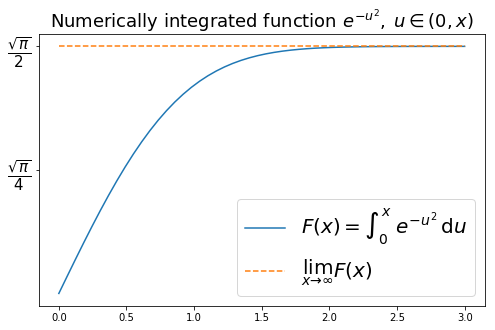
\includegraphics[width=0.7\textwidth]{function-F.png}
        \caption{Function $F(x)$ defined by \eqref{eq:F} obtained by numerical integration in Python. It can be shown {\itshape exactly} that $\lim\limits_{x \to \infty} F(x) = \sqrt{\pi}/2$.}
    \label{fig:F}
\end{figure}

\begin{figure}
    \centering
    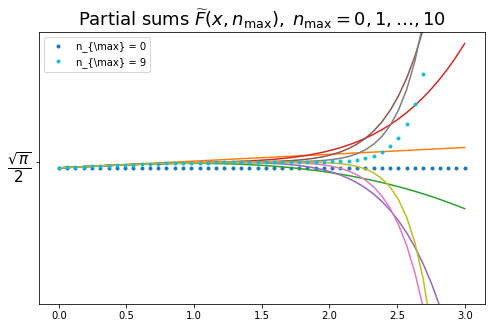
\includegraphics[width=0.7\textwidth]{function-F-tilde.png}
        \caption{Function $\widetilde{F}(x,n_{\max})$ defined by \eqref{eq:F-tilde} obtained by performing actually the sum for indicated values of $n_{\max}$.}
    \label{fig:F-tilde}
\end{figure}

To conclude this line of thoughts, some integrals or differential equations (or even other problems) do not admit a solution in the closed form. Can we consider solution in the form of infinite series \eqref{eq:Taylor-F} as a true, useful solution?

Well, one should realize that even many elementary functions can be, in fact calculated from the series of such kind, except for integer powers $x^n$. We are very familiar with sine or cosine because they have a good geometrical meaning and have been studied a lot, but in order to calculate, say $\sin 1.1$ we cannot resort directly to this geometrical meaning but we have to find the closest value to $1.1$ for which we can derive the value of sine geometrically and then perform a Taylor expansion around this point to reach $x=1.1$ with sufficient accuracy\footnote{Of course, in principle we can calculate {\itshape any value} $\sin x$ by expanding sine about zero, but then we have to sum up too many terms to make the method efficient and sufficiently precise.}.

Hence, our intuitive understanding of meaning of elementary function is important but otherwise it is just a kind of illusion that they are different from special functions like \eqref{eq:Taylor-F}. 

Moreover, also certain special functions appear in the context of physics or mathematics repetitively. \idxentry{Spherical harmonic functions}{functions!harmonic!spherical} appear naturally in problems with spherical symmetry{symmetry!spherical} like the angular part of \Schr equation{equation!\Schr} with spherical potential, in the study of rotational group{group!rotational}, adding angular momenta in quantum mechanics \idxentry{Fourier analysis}{Fourier!analysis} of the cosmic microwave background{cosmic microwave background}, etc. \idxentry{Bessel functions}{functions!Bessel} are typical for problems with \idxentry{cylindrical symmetry}{symmetry!cylindrical} (transfer of electromagnetic waves or heat in cylindrical objects) or with \idxentry{helical symmetry}{symmetry!helical} like DNA. \idxentry{Hypergeometric functions}{functions!hypergeometric} appear in \idxentry{statistics}{statistics}, in the integrals representing the \idxentry{Feynman diagrams}{Feynman!diagrams}.

\idxentry{Special functions}{functions!special} are functions which are not \idxentry{elementary}{functions!elementary}. However, we often use for \idxentry{Fourier series}{Fourier!series} functions which are in fact elementary but nevertheless call them special. For example, \idxentry{Legendre}{polynomials!Legendre} or \idxentry{Hermite}{polynomials!Hermite} are just pure polynomials of finite order. Such polynomials, if they solve the \idxentry{Sturm-Liouville problem}{problem!Sturm-Liouville}, form a \idxentry{complete}{set!complete} \idxentry{orthonormal}{set!orthonormal} of functions, meaning that any suitable function can be expanded into the (infinite) Fourier series of such polynomials. In contrast, polynomials $x^n$ do not have this property. Although any function can be expanded into a Taylor series, so that polynomials $x^n$ form a complete set, they are not orthogonal in any meaningful sense. The notion of orthogonality requires the presence of an additional structure, either \idxentry{norm}{norm} or \idxentry{inner product}{product!inner} and polynomials $x^n$ are not equipped with such structures. For these reasons we will call also orthogonal polynomials (like \idxentry{Legendre polynomials}{polynomials!Legendre}) special functions, although they are just ordinary elementary functions. 

%\chapter{Legendre polynomials}
\label{ch:legendre}


We start our exposition with \idxentry{Legendre polynomials}{polynomials!Legendre} and motivate them by \idxentry{multipole expansion}{expansion!multipole}. Roughly speaking multipole moments is an infinite set of numbers from which the structure of an isolated system can be reconstructed. It is an alternative description of the system and one way how to understand this is in terms of the \idxentry{Fourier series}{Fourier!series}

\section{Motivation: multipole expansion}

Recall that both in \idxentry{electrostatics}{electrostatics} and \idxentry{Newtonian theory of gravity}{gravity!Newtonian}, the \idxentry{point source}{source!point} has a potential inversely proportional to the distance from the source, the constant of proportionality being the \idxentry{mass}{mass} or the \idxentry{charge}{charge} of the source, respectively. Since electrostatics and Newtonian gravity behave exactly in the same way in this respect, for definiteness we will talk about the charges and \idxentry{electrostatic force}{force!electrostatic}, although we could freely replace them by mass and \idxentry{Newtonian gravitational force}{force!gravitational} (except for the cases when the sign of the charge pays a role but the reader that does not affect the core of the discussion).

However, real sources are \idxentry{extended}{source!extended}: they consist either of a system of point sources or they represent a continuous distribution of charge. In a special case of \idxentry{isolated source}{source!isolated}, the charges are distributed (discretely or continuously) in a finite domain -- we say that sources have a \idxentry{compact support}{support!compact}. 

For a very distant observer (in principle observer who is at infinity), such isolated source appears as a point source whose charge is given by the sum of charges of all source particles. As the observer approaches the source, the internal structure and distribution of the charges becomes more apparent. Imagine, for example a \idxentry{dipole}{dipole}, i.e.\ a system of two charges $+q$ and $-q$ at some fixed distance $d$. While each charge gives rise to a \idxentry{potential}{potential} proportional to $r^{-1}$, the net charge of the dipole vanishes and resulting potential decays as $r^{-2}$, that is, faster than the potential of each charge separately. However, when observer approaches the dipole, he will notice that the potential is non-vanishing, although weak, and he will notice attraction to one charge and repulsion from the other. 


\section{Monopole}
\label{sec:monopole}


Thus, the general setting is that there is a compact set $\DD$ of charges $q_i$. Choose the origin of the coordinate system $O$ somewhere in $\DD \ni O$ so that each charge has the \idxentry{position vector}{vector!position} $\bb{r}_i$ with respect to $O$. Potential of each charge is given by the distance $|\bb{r}-\bb{r}_i|$ where $\bb{r}$ is the position vector of a point $P$ lying outside (and typically sufficiently far from) $\DD$, see Figure \ref{fig:isolated-system}. Ignoring the physical constants, the total potential is
\begin{align}\label{eq:potential-sum}
    \phi(\bb{r}) &= \sum_{i}^N \frac{q_i}{|\bb{r}-\bb{r}_i|}\, ,
\end{align}
where $N$ is the number of charges in $\DD$, $\bb{r}_i$ is the position of $i$-th charge, $\bb{r}$ is the position of a distant observer and $\bb{r}-\bb{r}_i$ is the position of the observer with respect to $i$-th charge. 


\begin{figure}
    \centering
\begin{tikzpicture}[>=stealth,scale=2]
        \fill (0,0) circle(1pt) node[anchor=north east] {$O$};
        \draw[] (6pt,-2pt) node {$\theta_i$};
     
        \draw[->,dashed] (0,0) -- (80pt, 60pt) node[pos=0.5, sloped, above=1pt]
        {$\bb{r}$};
        
        
        
        \draw (80pt,60pt) node[anchor=south west] {$P$};
        \draw[dotted] (0, 0) circle (35pt);
        \draw (0, 33pt) node[anchor=south] {$\DD$};
        \draw[->,fill,dashed
        ] (0,0) -- (5pt, -25pt) node[anchor=east] {$\bb{r}_i$};
        \draw[->] (5pt, -25pt) -- (80pt,60pt) node[pos=0.5,sloped,below=-3pt] {$\bb{r}-\bb{r}_i$};
        
        %arc
        \draw[<->] (2.5pt,-12.5pt) arc (-78.7:37:12.74pt);
        
        %charges
        \draw[fill,blue] (5pt,-25pt) circle(0.5pt) node[anchor=north] {$q_i$};
        \draw[fill,blue] (-10pt,13pt) circle(0.5pt) node[anchor=east] {$q_j$};
        \draw[fill,blue] (-25pt,-15pt) circle(0.5pt) node[anchor=west] {$q_k$};
    \end{tikzpicture}    \caption{Isolated system of charges distributed in compact domain $\DD$ as seen by a far-away observer $P$.}
    \label{fig:isolated-system}
\end{figure}


If $r \gg r_i$, i.e.\ if we can neglect distance of charges from the origin compared to the distance of the observer, formula \eqref{eq:potential-sum} reduces to
\begin{align}\label{eq:potential-monopole}
    \phi(\bb{r}) &\approx \frac{\sum\limits_i q_i}{r} = \frac{Q}{r}\, , &
    Q = \sum_{i=1}^n q_i\, ,
\end{align}
where $Q$ is the total charge of isolated system. We talk about \idxentry{monopole}{monopole} (\idxentry{electric}{monopole!electric} or \idxentry{gravitational}{monopole!gravitational}) because in this approximation it behaves like a single point charge $Q$. The word \emph{monopole} refers to the fact that the lines of force emerge from (if the charge is positive) or end up at (if the charge is negative)  a single point.




Of course, general isolated system is not just monopole, but it always looks like monopole at sufficiently large distances. In order to probe the internal distribution of the charge in the domain $\DD$ we have to measure deviations from the monopole potential \eqref{eq:potential-monopole}. Mathematically, we have to expand \eqref{eq:potential-monopole} into the \idxentry{Taylor expansion}{expansion!Taylor!of the potential} in variables $\bb{r}_i$ (monopole is zeroth term in this expansion obtained simply by putting $\bb{r}_i=0$. For example, the first term of the expansion acquires the form 
\chapter{Spin-weighted spherical harmonics}
\label{ch:spin-weighted-harmonics}

We already know that \idxentry{spherical harmonics}{functions!harmonic!spherical}{spherical-harmonics}{spherical}
 \idxentry{spherical harmonics}{functions!harmonic!spherical}{spherical-harmonics}{spherical}




%%%%%%%%%%%%%%%

\printindex
\end{document}